

\section{$F$\textbf{-gauge choice}}

\begin{enumerate}
\item Explain why in the Fibonacci theory, $[F_{\tau }^{\tau \tau \tau } ]_{\tau \tau }$ is gauge independent but $[F_{\tau }^{\tau \tau \tau } ]_{I\tau }$ is gauge dependent.
\item Explain why in the Ising theory is $[F_{\sigma }^{\psi \sigma \psi } ]_{\sigma \sigma }$ is gauge independent, but $[F_{\psi }^{\sigma \psi \sigma } ]_{\sigma \sigma }$ is gauge dependent.
\end{enumerate}

\paragraph{Answer}
(a) In Fibonacci theory, consider the process $\tau ,\tau ,\tau $ fuse to $\tau $. We have:
\begin{equation*}
\begin{pmatrix}
|0\rangle \\
|1\rangle 
\end{pmatrix} =\begin{pmatrix}
[F_{\tau }^{\tau \tau \tau } ]_{II} & [F_{\tau }^{\tau \tau \tau } ]_{I\tau }\\
[F_{\tau }^{\tau \tau \tau } ]_{\tau I} & [F_{\tau }^{\tau \tau \tau } ]_{\tau \tau }
\end{pmatrix}\begin{pmatrix}
|0'\rangle \\
|1'\rangle 
\end{pmatrix} ,
\end{equation*}
where
\begin{equation*}
\tikzset{every picture/.style={line width=0.75pt}} %set default line width to 0.75pt        
\begin{tikzpicture}[x=0.75pt,y=0.75pt,yscale=-1,xscale=1, baseline=(XXXX.south) ]
\path (0,76);\path (92.9889907836914,0);\draw    ($(current bounding box.center)+(0,0.3em)$) node [anchor=south] (XXXX) {};
%Straight Lines [id:da6679856576688559] 
\draw [color={rgb, 255:red, 74; green, 144; blue, 226 }  ,draw opacity=1 ]   (1.56,14.56) -- (21,34) ;
%Straight Lines [id:da14116196892650712] 
\draw [color={rgb, 255:red, 74; green, 144; blue, 226 }  ,draw opacity=1 ]   (21,34) -- (41,14) ;
%Straight Lines [id:da8326498689328212] 
\draw [color={rgb, 255:red, 74; green, 144; blue, 226 }  ,draw opacity=1 ] [dash pattern={on 0.84pt off 2.51pt}]  (41,54) -- (21,34) ;
%Straight Lines [id:da7982058810830115] 
\draw [color={rgb, 255:red, 74; green, 144; blue, 226 }  ,draw opacity=1 ]   (81,14) -- (21,74) ;
% Text Node
\draw (2,-3.5) node [anchor=north west][inner sep=0.75pt]    {$\tau $};
% Text Node
\draw (42,-3.5) node [anchor=north west][inner sep=0.75pt]    {$\tau $};
% Text Node
\draw (82,-3.5) node [anchor=north west][inner sep=0.75pt]    {$\tau $};
% Text Node
\draw (9,56.5) node [anchor=north west][inner sep=0.75pt]    {$\tau $};
% Text Node
\draw (33,25.5) node [anchor=north west][inner sep=0.75pt]    {$I$};
\end{tikzpicture}
=|0\rangle ,\quad \tikzset{every picture/.style={line width=0.75pt}} %set default line width to 0.75pt        
\begin{tikzpicture}[x=0.75pt,y=0.75pt,yscale=-1,xscale=1, baseline=(XXXX.south) ]
\path (0,76);\path (92.9889907836914,0);\draw    ($(current bounding box.center)+(0,0.3em)$) node [anchor=south] (XXXX) {};
%Straight Lines [id:da23482911055376698] 
\draw [color={rgb, 255:red, 74; green, 144; blue, 226 }  ,draw opacity=1 ]   (2.55,13.54) -- (41.99,52.98) ;
%Straight Lines [id:da5187919992908567] 
\draw [color={rgb, 255:red, 74; green, 144; blue, 226 }  ,draw opacity=1 ]   (21.99,32.98) -- (41.99,12.98) ;
%Straight Lines [id:da6132340599706072] 
\draw [color={rgb, 255:red, 74; green, 144; blue, 226 }  ,draw opacity=1 ]   (81.99,12.98) -- (21.99,72.98) ;
% Text Node
\draw (2.99,-4.52) node [anchor=north west][inner sep=0.75pt]    {$\tau $};
% Text Node
\draw (42.99,-4.52) node [anchor=north west][inner sep=0.75pt]    {$\tau $};
% Text Node
\draw (82.99,-4.52) node [anchor=north west][inner sep=0.75pt]    {$\tau $};
% Text Node
\draw (9.99,55.48) node [anchor=north west][inner sep=0.75pt]    {$\tau $};
% Text Node
\draw (33.99,24.48) node [anchor=north west][inner sep=0.75pt]    {$\tau $};
\end{tikzpicture}
=|1\rangle .
\end{equation*}
Now we consider a gauge transformation on the vertices. According to the transformation rule of $F$, if the on one vertex, the gauge transformation is given by:
\begin{equation*}
\tikzset{every picture/.style={line width=0.75pt}} %set default line width to 0.75pt        
\begin{tikzpicture}[x=0.75pt,y=0.75pt,yscale=-1,xscale=1, baseline=(XXXX.south) ]
\path (0,50);\path (43.98124313354492,0);\draw    ($(current bounding box.center)+(0,0.3em)$) node [anchor=south] (XXXX) {};
%Straight Lines [id:da6721611237810059] 
\draw [color={rgb, 255:red, 74; green, 144; blue, 226 }  ,draw opacity=1 ]   (2,8) -- (22,28) ;
%Straight Lines [id:da27101694568404877] 
\draw [color={rgb, 255:red, 74; green, 144; blue, 226 }  ,draw opacity=1 ]   (22,28) -- (42,8) ;
%Straight Lines [id:da24019406696757506] 
\draw [color={rgb, 255:red, 74; green, 144; blue, 226 }  ,draw opacity=1 ]   (22,48) -- (22,28) ;
% Text Node
\draw (6,0) node [anchor=north west][inner sep=0.75pt]    {$a$};
% Text Node
\draw (26.99,-3) node [anchor=north west][inner sep=0.75pt]    {$b$};
% Text Node
\draw (24,29.5) node [anchor=north west][inner sep=0.75pt]    {$c$};
\end{tikzpicture}
=u_{c}^{ab}\tikzset{every picture/.style={line width=0.75pt}} %set default line width to 0.75pt        
\begin{tikzpicture}[x=0.75pt,y=0.75pt,yscale=-1,xscale=1, baseline=(XXXX.south) ]
\path (0,50);\path (43.98124313354492,0);\draw    ($(current bounding box.center)+(0,0.3em)$) node [anchor=south] (XXXX) {};
%Straight Lines [id:da5541944561024958] 
\draw [color={rgb, 255:red, 74; green, 144; blue, 226 }  ,draw opacity=1 ]   (2,8) -- (22,28) ;
%Straight Lines [id:da395643263838791] 
\draw [color={rgb, 255:red, 74; green, 144; blue, 226 }  ,draw opacity=1 ]   (22,28) -- (42,8) ;
%Straight Lines [id:da8544980505411282] 
\draw [color={rgb, 255:red, 74; green, 144; blue, 226 }  ,draw opacity=1 ]   (22,48) -- (22,28) ;
% Text Node
\draw (6,0) node [anchor=north west][inner sep=0.75pt]    {$a$};
% Text Node
\draw (26.99,-3) node [anchor=north west][inner sep=0.75pt]    {$b$};
% Text Node
\draw (24,29.5) node [anchor=north west][inner sep=0.75pt]    {$c$};
% Text Node
\draw (14.97,8.5) node [anchor=north west][inner sep=0.75pt]  [color={rgb, 255:red, 74; green, 144; blue, 226 }  ,opacity=1 ]  {$\widetilde{\ \ \ }$};
\end{tikzpicture}
,
\end{equation*}
then
\begin{equation*}
[\tilde{F}_{e}^{abc} ]_{df} =\frac{u_{e}^{af} u_{f}^{bc}}{u_{d}^{ab} u_{e}^{dc}} [F_{e}^{abc} ]_{df} .
\end{equation*}
Also note that if one of the upper legs is the identity, we typically do not allow a gauge transform of this type of vertex, i.e.
\begin{equation*}
u_{\tau }^{I\tau } =1.
\end{equation*}
Then
\begin{equation*}
[\tilde{F}_{\tau }^{\tau \tau \tau } ]_{\tau \tau } =\frac{u_{\tau }^{\tau \tau } u_{\tau }^{\tau \tau }}{u_{\tau }^{\tau \tau } u_{\tau }^{\tau \tau }} [F_{\tau }^{\tau \tau \tau } ]_{\tau \tau } =[F_{\tau }^{\tau \tau \tau } ]_{\tau \tau } ,
\end{equation*}
which means $[F_{\tau }^{\tau \tau \tau } ]_{\tau \tau }$ is gauge independent. But for
\begin{equation*}
[\tilde{F}_{\tau }^{\tau \tau \tau } ]_{I\tau } =\frac{u_{\tau }^{\tau \tau } u_{\tau }^{\tau \tau }}{u_{I}^{\tau \tau } u_{\tau }^{\tau \tau }} [F_{\tau }^{\tau \tau \tau } ]_{I\tau } =u_{\tau }^{\tau \tau } [F_{\tau }^{\tau \tau \tau } ]_{I\tau } ,
\end{equation*}
which means $[F_{\tau }^{\tau \tau \tau } ]_{I\tau }$ is gauge dependent. 



(b) For Ising, the case is the same:
\begin{equation*}
[\tilde{F}_{\sigma }^{\psi \sigma \psi } ]_{\sigma \sigma } =\frac{u_{\sigma }^{\psi \sigma } u_{\sigma }^{\sigma \psi }}{u_{\sigma }^{\psi \sigma } u_{\sigma }^{\sigma \psi }} [F_{\sigma }^{\psi \sigma \psi } ]_{\sigma \sigma } =[F_{\sigma }^{\psi \sigma \psi } ]_{\sigma \sigma } ,
\end{equation*}
which means $[F_{\sigma }^{\psi \sigma \psi } ]_{\sigma \sigma }$ is gauge independent. While
\begin{equation*}
[\tilde{F}_{\psi }^{\sigma \psi \sigma } ]_{\sigma \sigma } =\ \frac{u_{\psi }^{\sigma \sigma } u_{\sigma }^{\psi \sigma }}{u_{\sigma }^{\sigma \psi } u_{\psi }^{\sigma \sigma }} [F_{\psi }^{\sigma \psi \sigma } ]_{\sigma \sigma } =\frac{u_{\sigma }^{\psi \sigma }}{u_{\sigma }^{\sigma \psi }} [F_{\psi }^{\sigma \psi \sigma } ]_{\sigma \sigma } ,
\end{equation*}
which means $[F_{\psi }^{\sigma \psi \sigma } ]_{\sigma \sigma }$ is gauge dependent. Note that $u_{c}^{ab} \neq u_{c}^{ba}$ in general. 

\section{$F$\textbf{'s with the vacuum field }$I$}
Explain why $[F_{e}^{aIc} ]_{ac} =[F_{d}^{abI} ]_{db} =[F_{e}^{Ibc} ]_{be} =1$.

\paragraph{Answer}
We first prove $[F_{e}^{aIc} ]_{ac}$ is gauge invariant:
\begin{equation*}
[\tilde{F}_{e}^{aIc} ]_{ac} =\frac{u_{e}^{ac} u_{c}^{Ic}}{u_{a}^{aI} u_{e}^{ac}} [F_{e}^{aIc} ]_{ac} =[F_{e}^{aIc} ]_{ac} .
\end{equation*}
Then draw the tree:
\begin{equation*}
\tikzset{every picture/.style={line width=0.75pt}} %set default line width to 0.75pt        
\begin{tikzpicture}[x=0.75pt,y=0.75pt,yscale=-1,xscale=1, baseline=(XXXX.south) ]
\path (0,76);\path (95.9889907836914,0);\draw    ($(current bounding box.center)+(0,0.3em)$) node [anchor=south] (XXXX) {};
%Straight Lines [id:da31833903758109505] 
\draw [color={rgb, 255:red, 74; green, 144; blue, 226 }  ,draw opacity=1 ]   (4,15) -- (44,55) ;
%Straight Lines [id:da9988250019768812] 
\draw [color={rgb, 255:red, 74; green, 144; blue, 226 }  ,draw opacity=1 ] [dash pattern={on 0.84pt off 2.51pt}]  (24,35) -- (44,15) ;
%Straight Lines [id:da24713558775014] 
\draw [color={rgb, 255:red, 74; green, 144; blue, 226 }  ,draw opacity=1 ]   (24,75) -- (84,15) ;
% Text Node
\draw (5,-2.5) node [anchor=north west][inner sep=0.75pt]    {$a$};
% Text Node
\draw (45,-2.5) node [anchor=north west][inner sep=0.75pt]    {$I$};
% Text Node
\draw (85,-2.5) node [anchor=north west][inner sep=0.75pt]    {$c$};
% Text Node
\draw (15,55.5) node [anchor=north west][inner sep=0.75pt]    {$e$};
% Text Node
\draw (36,26.5) node [anchor=north west][inner sep=0.75pt]    {$a$};
\end{tikzpicture}
=[F_{e}^{aIc} ]_{ac}\tikzset{every picture/.style={line width=0.75pt}} %set default line width to 0.75pt        
\begin{tikzpicture}[x=0.75pt,y=0.75pt,yscale=-1,xscale=1, baseline=(XXXX.south) ]
\path (0,76);\path (95.9889907836914,0);\draw    ($(current bounding box.center)+(0,0.3em)$) node [anchor=south] (XXXX) {};
%Straight Lines [id:da8447066740979126] 
\draw [color={rgb, 255:red, 74; green, 144; blue, 226 }  ,draw opacity=1 ]   (2.99,18.99) -- (42.99,58.99) ;
%Straight Lines [id:da1909051258290011] 
\draw [color={rgb, 255:red, 74; green, 144; blue, 226 }  ,draw opacity=1 ] [dash pattern={on 0.84pt off 2.51pt}]  (62.99,38.99) -- (42.99,18.99) ;
%Straight Lines [id:da0037491210175448764] 
\draw [color={rgb, 255:red, 74; green, 144; blue, 226 }  ,draw opacity=1 ]   (22.99,78.99) -- (82.99,18.99) ;
% Text Node
\draw (3.99,1.49) node [anchor=north west][inner sep=0.75pt]    {$a$};
% Text Node
\draw (43.99,1.49) node [anchor=north west][inner sep=0.75pt]    {$I$};
% Text Node
\draw (83.99,1.49) node [anchor=north west][inner sep=0.75pt]    {$c$};
% Text Node
\draw (13.99,59.49) node [anchor=north west][inner sep=0.75pt]    {$e$};
% Text Node
\draw (40.99,31.49) node [anchor=north west][inner sep=0.75pt]    {$c$};
\end{tikzpicture}
=\tikzset{every picture/.style={line width=0.75pt}} %set default line width to 0.75pt        
\begin{tikzpicture}[x=0.75pt,y=0.75pt,yscale=-1,xscale=1, baseline=(XXXX.south) ]
\path (0,55);\path (42.930747985839844,0);\draw    ($(current bounding box.center)+(0,0.3em)$) node [anchor=south] (XXXX) {};
%Straight Lines [id:da352670813916768] 
\draw [color={rgb, 255:red, 74; green, 144; blue, 226 }  ,draw opacity=1 ]   (1,12) -- (21,32) ;
%Straight Lines [id:da47740644842639646] 
\draw [color={rgb, 255:red, 74; green, 144; blue, 226 }  ,draw opacity=1 ]   (21,32) -- (41,12) ;
%Straight Lines [id:da3543986158283676] 
\draw [color={rgb, 255:red, 74; green, 144; blue, 226 }  ,draw opacity=1 ]   (21,32) -- (21,52) ;
% Text Node
\draw (2,-5.5) node [anchor=north west][inner sep=0.75pt]    {$a$};
% Text Node
\draw (29,-5.5) node [anchor=north west][inner sep=0.75pt]    {$c$};
% Text Node
\draw (2,34.5) node [anchor=north west][inner sep=0.75pt]    {$e$};
\end{tikzpicture}
,
\end{equation*}
we can see the identity can be omitted, which means they are actually the same process, namely
\begin{equation*}
[F_{e}^{aIc} ]_{ac} =1.
\end{equation*}
For $[F_{d}^{abI} ]_{db} ,[F_{e}^{Ibc} ]_{be}$, the argument is the same. 

\section{Ising Pentagon}
Consider a system of Ising anyons. Given the fusion rules, $F_{w}^{xyz}$ will be a 2 by 2 matrix in the case of $x=y=z=w=\sigma $ (given by Eq. 9.4) and is a simply a scalar otherwise. One might hope that these scalars can all be taken to be unity. Unfortunately this is not the case. By examining the pentagon equation, Eq. $9.7$ in the case of $a=b=c=\sigma $ and $d=f=\psi $ show that taking the scalar to always be unity is not consistent. Show further that choosing $[F_{\sigma }^{\psi \sigma \psi } ]_{\sigma \sigma } =-1$ (and leaving the other scalars to be unity) allows a consistent solution of the pentagon for $a=b=c=\sigma $ and $d=f=\psi $.

\paragraph{Answer}
We give the pentagon identity:
\begin{equation*}
[F_{e}^{fcd} ]_{gl} [F_{e}^{abl} ]_{fk} =\sum _{h} [F_{g}^{abc} ]_{fh} [F_{e}^{ahd} ]_{gk} [F_{k}^{bcd} ]_{hl} .
\end{equation*}
with $a=b=c=\sigma $ and $d=f=\psi $, we have:
\begin{equation*}
[F_{\sigma }^{\psi \sigma \psi } ]_{\sigma \sigma } \cdot [F_{\sigma }^{\sigma \sigma \sigma } ]_{\psi k} =\sum _{h} [F_{\sigma }^{\sigma \sigma \sigma } ]_{\psi h} [F_{\sigma }^{\sigma h\psi } ]_{\sigma k} [F_{k}^{\sigma \sigma \psi } ]_{h\sigma } .
\end{equation*}
However, for process $F_{\sigma }^{\sigma h\psi }$, we must have $h=\psi $ because if $h=\sigma $, $\sigma \times \sigma =I+\psi $, while $( I+\psi ) \times \psi $ cannot give $\sigma $. So
\begin{equation*}
[F_{\sigma }^{\psi \sigma \psi } ]_{\sigma \sigma } \cdot [F_{\sigma }^{\sigma \sigma \sigma } ]_{\psi k} =[F_{\sigma }^{\sigma \sigma \sigma } ]_{\psi \psi } [F_{\sigma }^{\sigma \psi \psi } ]_{\sigma k} [F_{k}^{\sigma \sigma \psi } ]_{\psi \sigma } .
\end{equation*}
For the term $F_{\sigma }^{\sigma \psi \psi }$, the only possible $k$ is $k=I$ because $\psi \times \psi =I$. In this case:
\begin{equation*}
\mathrm{LHS} =[F_{\sigma }^{\psi \sigma \psi } ]_{\sigma \sigma } \cdot [F_{\sigma }^{\sigma \sigma \sigma } ]_{\psi I} =[F_{\sigma }^{\psi \sigma \psi } ]_{\sigma \sigma } \cdot \frac{1}{\sqrt{2}} ,
\end{equation*}
while
\begin{equation*}
\mathrm{RHS} =-\frac{1}{\sqrt{2}} \cdot [F_{\sigma }^{\sigma \psi \psi } ]_{\sigma I} \cdot [F_{I}^{\sigma \sigma \psi } ]_{\psi \sigma } .
\end{equation*}
If we choose $[F_{\sigma }^{\psi \sigma \psi } ]_{\sigma \sigma } =[F_{\sigma }^{\sigma \psi \psi } ]_{\sigma I} =[F_{I}^{\sigma \sigma \psi } ]_{\psi \sigma }$(because $F_{I}^{\sigma \sigma \psi } ,F_{\sigma }^{\sigma \psi \psi }$ are also scalar), the equality cannot hold, which means that taking the scalar to always be unity is not consistent. 



Now, if we leave the scalar $F_{I}^{\sigma \sigma \psi } ,F_{\sigma }^{\sigma \psi \psi }$ to be unity and choose $[F_{\sigma }^{\psi \sigma \psi } ]_{\sigma \sigma } =-1$, then
\begin{equation*}
\mathrm{LHS} =[F_{\sigma }^{\psi \sigma \psi } ]_{\sigma \sigma } \cdot \frac{1}{\sqrt{2}} =-\frac{1}{\sqrt{2}} ,
\end{equation*}
while
\begin{equation*}
\mathrm{RHS} =-\frac{1}{\sqrt{2}} \cdot [F_{\sigma }^{\sigma \psi \psi } ]_{\sigma I} \cdot [F_{I}^{\sigma \sigma \psi } ]_{\psi \sigma } =-\frac{1}{\sqrt{2}} =\mathrm{LHS} ,
\end{equation*}
which is consistent, thus allowing a consistent solution of the pentagon for $a=b=c=\sigma $ and $d=f=\psi $.

\section{Fibonacci Pentagon}
In the Fibonacci anyon model, there are two particle types which are usually called $I$ and $\tau $. The only nontrivial fusion rule is $\tau \times \tau =I+\tau $. With these fusion rules, the $F$-matrix is completely fixed up to a gauge freedom (corresponding to adding a phase to some of the kets). If we choose all elements of the $F$-matrix to be real, then the $F$-matrix is completely determined by the pentagon up to one sign (gauge) choice. Using the pentagon equation determine the $F$-matrix. (To get you started, note that in Fig. $9.7$ the variables $a,b,c,d,e,f,g,h$ can only take values $I$ and $\tau $. You only need to consider the cases where $a,b,c,d$ are all $\tau $ ).

If you are stuck as to how to start, part of the calculation is given in Nayak et al. [2008].

\paragraph{Answer}
Before we look at the pentagon identity, consider the only nontrivial matrix $F_{\tau }^{\tau \tau \tau }$:
\begin{equation*}
F_{\tau }^{\tau \tau \tau } =\begin{pmatrix}
(F_{\tau }^{\tau \tau \tau } )_{II} & (F_{\tau }^{\tau \tau \tau } )_{I\tau }\\
(F_{\tau }^{\tau \tau \tau } )_{\tau I} & (F_{\tau }^{\tau \tau \tau } )_{\tau \tau }
\end{pmatrix} \equiv \begin{pmatrix}
F_{00} & F_{01}\\
F_{10} & F_{11}
\end{pmatrix} .
\end{equation*}
We can choose this basis transform to be unitary and real, i.e.
\begin{equation*}
\begin{pmatrix}
F_{00}^{2} +F_{01}^{2} & F_{00} F_{10} +F_{01} F_{11}\\
F_{10} F_{00} +F_{11} F_{01} & F_{10}^{2} +F_{11}^{2}
\end{pmatrix} =\begin{pmatrix}
1 & 0\\
0 & 1
\end{pmatrix} .
\end{equation*}
Now we consider the case $a=b=l=f=c=d=g=k=\tau $, while $e=I$, this gives
\begin{equation*}
[F_{I}^{\tau \tau \tau } ]_{\tau \tau } [F_{I}^{\tau \tau \tau } ]_{\tau \tau } =[F_{\tau }^{\tau \tau \tau } ]_{\tau \tau } [F_{I}^{\tau \tau \tau } ]_{\tau \tau } [F_{\tau }^{\tau \tau \tau } ]_{\tau \tau } +[F_{\tau }^{\tau \tau \tau } ]_{\tau I} [F_{I}^{\tau I\tau } ]_{\tau \tau } [F_{\tau }^{\tau \tau \tau } ]_{I\tau } .
\end{equation*}
However, we know $F_{I}^{\tau \tau \tau } =F_{I}^{\tau I\tau } =1$ because in the second case, one of the upper indice is the identity. This gives
\begin{equation*}
1=F_{11}^{2} +F_{10} F_{01} .
\end{equation*}
Now with
\begin{equation*}
F_{10}^{2} +F_{11}^{2} =1,
\end{equation*}
we have $F_{10} =F_{01}$, which means we also have
\begin{equation*}
F_{00}^{2} =F_{11}^{2} =1-F_{01}^{2} .
\end{equation*}
Now we take $a=b=c=d=\tau $, and choose $e=f=g=k=l=\tau $, which gives
\begin{equation*}
(F_{\tau }^{\tau \tau \tau } )^{2} =(F_{\tau }^{\tau \tau \tau } )_{\tau \tau }^{2} (F_{\tau }^{\tau \tau \tau } )_{\tau \tau } +(F_{\tau }^{\tau \tau \tau } )_{\tau I} (F_{\tau }^{\tau \tau \tau } )_{\tau \tau } (F_{\tau }^{\tau \tau \tau } )_{I\tau } ,
\end{equation*}
i.e.
\begin{equation*}
F_{11}^{2} =F_{11}^{3} +F_{01}^{2} =F_{11}^{3} +1-F_{11}^{2} .
\end{equation*}
This equation have three roots: $F_{11} =1$, $F_{11} =(\sqrt{5} +1)/2$ or $F_{11} =(-\sqrt{5} +1)/2$. According to the reality condition and $F_{01}^{2} =1-F_{11}^{2}$, the second root is ruled out. 

Finally we choose $e=f=k=\tau $, while $g=l=I$, we can see
\begin{equation*}
F_{00} =F_{01}^{2} .
\end{equation*}
Now with $F_{00}^{2} =F_{11}^{2}$, the root $F_{11} =1$ can be also excluded. So we finally have
\begin{equation*}
F_{00} =-F_{11} =\frac{\sqrt{5} -1}{2} ,
\end{equation*}
while $F_{01} =F_{10} =F_{00}^{1/2}$ for one gauge, i.e.
\begin{equation*}
F_{\tau }^{\tau \tau \tau } =\begin{pmatrix}
\phi ^{-1} & \phi ^{-1/2}\\
\phi ^{-1/2} & -\phi 
\end{pmatrix} ,
\end{equation*}
where $\phi =(1+\sqrt{5} )/2$ is the golden ratio. 

\section{Pentagon and Fusion Multiplicities}
Consider the case of Appendix $9.5.3$ where there are fusion multiplicies $N_{ab}^{c}  >1$. Write the generalization of the pentagon equation Eq. 9.7.

\paragraph{Answer}
With $N_{ab}^{c}  >1$, the $F$ matrix between these three anyons are given by:
\begin{equation*}
\tikzset{every picture/.style={line width=0.75pt}} %set default line width to 0.75pt        
\begin{tikzpicture}[x=0.75pt,y=0.75pt,yscale=-1,xscale=1, baseline=(XXXX.south) ]
\path (0,75);\path (92.97021484375,0);\draw    ($(current bounding box.center)+(0,0.3em)$) node [anchor=south] (XXXX) {};
%Straight Lines [id:da4920197522533427] 
\draw [color={rgb, 255:red, 74; green, 144; blue, 226 }  ,draw opacity=1 ]   (12,9) -- (52,49) ;
%Straight Lines [id:da4388784373180308] 
\draw [color={rgb, 255:red, 74; green, 144; blue, 226 }  ,draw opacity=1 ]   (32,29) -- (52,9) ;
%Straight Lines [id:da06563557562582667] 
\draw [color={rgb, 255:red, 74; green, 144; blue, 226 }  ,draw opacity=1 ]   (32,69) -- (92,9) ;
%Straight Lines [id:da16022077648655886] 
\draw [color={rgb, 255:red, 208; green, 2; blue, 27 }  ,draw opacity=1 ]   (32,29) ;
\draw [shift={(32,29)}, rotate = 0] [color={rgb, 255:red, 208; green, 2; blue, 27 }  ,draw opacity=1 ][fill={rgb, 255:red, 208; green, 2; blue, 27 }  ,fill opacity=1 ][line width=0.75]      (0, 0) circle [x radius= 2.01, y radius= 2.01]   ;
%Straight Lines [id:da5526849872942077] 
\draw [color={rgb, 255:red, 208; green, 2; blue, 27 }  ,draw opacity=1 ]   (52,49) ;
\draw [shift={(52,49)}, rotate = 0] [color={rgb, 255:red, 208; green, 2; blue, 27 }  ,draw opacity=1 ][fill={rgb, 255:red, 208; green, 2; blue, 27 }  ,fill opacity=1 ][line width=0.75]      (0, 0) circle [x radius= 2.01, y radius= 2.01]   ;
% Text Node
\draw (0,-0.5) node [anchor=north west][inner sep=0.75pt]    {$a$};
% Text Node
\draw (33,-0.5) node [anchor=north west][inner sep=0.75pt]    {$b$};
% Text Node
\draw (80,-0.5) node [anchor=north west][inner sep=0.75pt]    {$c$};
% Text Node
\draw (33,39.5) node [anchor=north west][inner sep=0.75pt]    {$f$};
% Text Node
\draw (42,59) node [anchor=north west][inner sep=0.75pt]    {$g$};
% Text Node
\draw (13,21.5) node [anchor=north west][inner sep=0.75pt]  [color={rgb, 255:red, 208; green, 2; blue, 27 }  ,opacity=1 ]  {$\mu $};
% Text Node
\draw (60,41.5) node [anchor=north west][inner sep=0.75pt]  [color={rgb, 255:red, 208; green, 2; blue, 27 }  ,opacity=1 ]  {$\nu $};
\end{tikzpicture}
=\sum _{h,\alpha ,\beta } [F_{g}^{abc} ]_{( f\mu \nu )( h\alpha \beta )}\tikzset{every picture/.style={line width=0.75pt}} %set default line width to 0.75pt        
\begin{tikzpicture}[x=0.75pt,y=0.75pt,yscale=-1,xscale=1, baseline=(XXXX.south) ]
\path (0,75);\path (92.97021484375,0);\draw    ($(current bounding box.center)+(0,0.3em)$) node [anchor=south] (XXXX) {};
%Straight Lines [id:da8708000090493899] 
\draw [color={rgb, 255:red, 74; green, 144; blue, 226 }  ,draw opacity=1 ]   (11.97,8.96) -- (51.97,48.96) ;
%Straight Lines [id:da9507746762108156] 
\draw [color={rgb, 255:red, 74; green, 144; blue, 226 }  ,draw opacity=1 ]   (71.97,28.96) -- (51.97,8.96) ;
%Straight Lines [id:da5524349961873474] 
\draw [color={rgb, 255:red, 74; green, 144; blue, 226 }  ,draw opacity=1 ]   (31.97,68.96) -- (91.97,8.96) ;
%Straight Lines [id:da0774062191362832] 
\draw [color={rgb, 255:red, 208; green, 2; blue, 27 }  ,draw opacity=1 ]   (71.97,28.96) ;
\draw [shift={(71.97,28.96)}, rotate = 0] [color={rgb, 255:red, 208; green, 2; blue, 27 }  ,draw opacity=1 ][fill={rgb, 255:red, 208; green, 2; blue, 27 }  ,fill opacity=1 ][line width=0.75]      (0, 0) circle [x radius= 2.01, y radius= 2.01]   ;
%Straight Lines [id:da7519162142441365] 
\draw [color={rgb, 255:red, 208; green, 2; blue, 27 }  ,draw opacity=1 ]   (51.97,48.96) ;
\draw [shift={(51.97,48.96)}, rotate = 0] [color={rgb, 255:red, 208; green, 2; blue, 27 }  ,draw opacity=1 ][fill={rgb, 255:red, 208; green, 2; blue, 27 }  ,fill opacity=1 ][line width=0.75]      (0, 0) circle [x radius= 2.01, y radius= 2.01]   ;
% Text Node
\draw (80,-0.5) node [anchor=north west][inner sep=0.75pt]    {$c$};
% Text Node
\draw (-0.03,-0.54) node [anchor=north west][inner sep=0.75pt]    {$a$};
% Text Node
\draw (32.97,-0.54) node [anchor=north west][inner sep=0.75pt]    {$b$};
% Text Node
\draw (52.97,21.46) node [anchor=north west][inner sep=0.75pt]    {$h$};
% Text Node
\draw (41.97,59) node [anchor=north west][inner sep=0.75pt]    {$g$};
% Text Node
\draw (79.97,21.46) node [anchor=north west][inner sep=0.75pt]  [color={rgb, 255:red, 208; green, 2; blue, 27 }  ,opacity=1 ]  {$\alpha $};
% Text Node
\draw (59.97,41.46) node [anchor=north west][inner sep=0.75pt]  [color={rgb, 255:red, 208; green, 2; blue, 27 }  ,opacity=1 ]  {$\beta $};
\end{tikzpicture}
.
\end{equation*}
Then the pentagon diagram looks like Fig.\ref{fig:pentagonWithMultiplicity}.

\begin{figure}[h!]
\centering
\tikzset{every picture/.style={line width=0.75pt}} %set default line width to 0.75pt        

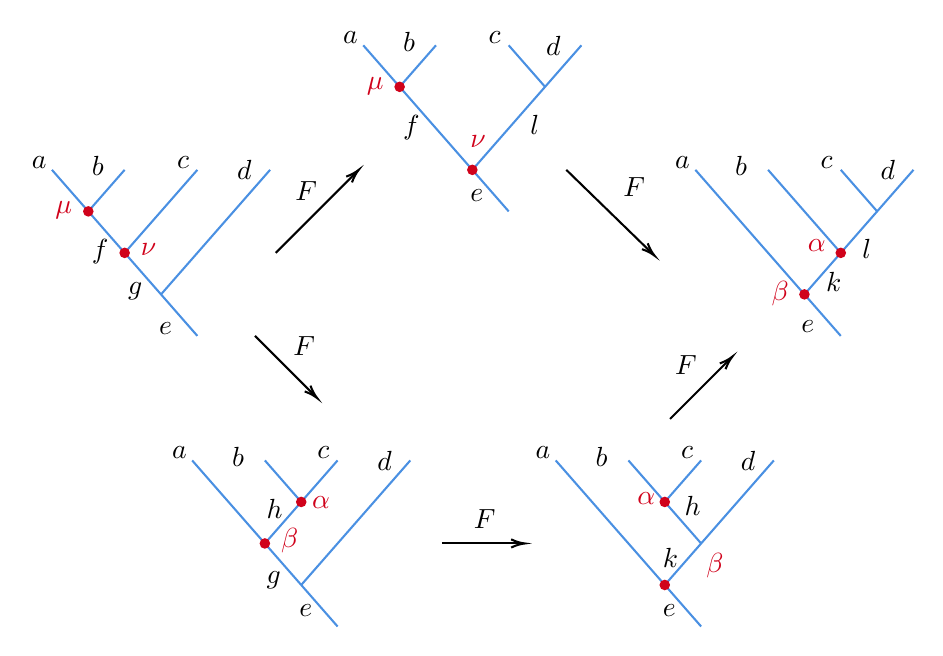
\begin{tikzpicture}[x=0.75pt,y=0.75pt,yscale=-1,xscale=1]
%uncomment if require: \path (0,294); %set diagram left start at 0, and has height of 294

%Straight Lines [id:da15061923928767573] 
\draw [color={rgb, 255:red, 74; green, 144; blue, 226 }  ,draw opacity=1 ]   (424.45,272) -- (477,212) ;
%Straight Lines [id:da5216466568167186] 
\draw [color={rgb, 255:red, 74; green, 144; blue, 226 }  ,draw opacity=1 ]   (331.74,72) -- (384.29,12) ;
%Straight Lines [id:da0898255957195595] 
\draw [color={rgb, 255:red, 74; green, 144; blue, 226 }  ,draw opacity=1 ]   (491.74,132) -- (544.29,72) ;
%Straight Lines [id:da12288457714289369] 
\draw [color={rgb, 255:red, 74; green, 144; blue, 226 }  ,draw opacity=1 ]   (129.19,72) -- (199.25,152) ;
%Straight Lines [id:da9990301087017979] 
\draw [color={rgb, 255:red, 74; green, 144; blue, 226 }  ,draw opacity=1 ]   (146.71,92) -- (164.22,72) ;
%Straight Lines [id:da465063761794523] 
\draw [color={rgb, 255:red, 74; green, 144; blue, 226 }  ,draw opacity=1 ]   (164.22,112) -- (199.25,72) ;
%Straight Lines [id:da21519014232208455] 
\draw [color={rgb, 255:red, 208; green, 2; blue, 27 }  ,draw opacity=1 ]   (146.71,92) ;
\draw [shift={(146.71,92)}, rotate = 0] [color={rgb, 255:red, 208; green, 2; blue, 27 }  ,draw opacity=1 ][fill={rgb, 255:red, 208; green, 2; blue, 27 }  ,fill opacity=1 ][line width=0.75]      (0, 0) circle [x radius= 2.01, y radius= 2.01]   ;
%Straight Lines [id:da29922676669019865] 
\draw [color={rgb, 255:red, 208; green, 2; blue, 27 }  ,draw opacity=1 ]   (164.22,112) ;
\draw [shift={(164.22,112)}, rotate = 0] [color={rgb, 255:red, 208; green, 2; blue, 27 }  ,draw opacity=1 ][fill={rgb, 255:red, 208; green, 2; blue, 27 }  ,fill opacity=1 ][line width=0.75]      (0, 0) circle [x radius= 2.01, y radius= 2.01]   ;
%Straight Lines [id:da610030043706981] 
\draw [color={rgb, 255:red, 74; green, 144; blue, 226 }  ,draw opacity=1 ]   (181.74,132) -- (234.29,72) ;
%Straight Lines [id:da3774190769439427] 
\draw [color={rgb, 255:red, 74; green, 144; blue, 226 }  ,draw opacity=1 ]   (279.19,12) -- (349.25,92) ;
%Straight Lines [id:da3810977475869053] 
\draw [color={rgb, 255:red, 74; green, 144; blue, 226 }  ,draw opacity=1 ]   (296.71,32) -- (314.22,12) ;
%Straight Lines [id:da2526511260014692] 
\draw [color={rgb, 255:red, 74; green, 144; blue, 226 }  ,draw opacity=1 ]   (366.77,32) -- (349.25,12) ;
%Straight Lines [id:da6162970945726176] 
\draw [color={rgb, 255:red, 208; green, 2; blue, 27 }  ,draw opacity=1 ]   (296.71,32) ;
\draw [shift={(296.71,32)}, rotate = 0] [color={rgb, 255:red, 208; green, 2; blue, 27 }  ,draw opacity=1 ][fill={rgb, 255:red, 208; green, 2; blue, 27 }  ,fill opacity=1 ][line width=0.75]      (0, 0) circle [x radius= 2.01, y radius= 2.01]   ;
%Straight Lines [id:da02189491360800022] 
\draw [color={rgb, 255:red, 208; green, 2; blue, 27 }  ,draw opacity=1 ]   (331.74,72) ;
\draw [shift={(331.74,72)}, rotate = 0] [color={rgb, 255:red, 208; green, 2; blue, 27 }  ,draw opacity=1 ][fill={rgb, 255:red, 208; green, 2; blue, 27 }  ,fill opacity=1 ][line width=0.75]      (0, 0) circle [x radius= 2.01, y radius= 2.01]   ;
%Straight Lines [id:da022116496210201175] 
\draw [color={rgb, 255:red, 74; green, 144; blue, 226 }  ,draw opacity=1 ]   (439.19,72) -- (509.25,152) ;
%Straight Lines [id:da29931560748895003] 
\draw [color={rgb, 255:red, 74; green, 144; blue, 226 }  ,draw opacity=1 ]   (509.25,112) -- (474.22,72) ;
%Straight Lines [id:da2788593835829203] 
\draw [color={rgb, 255:red, 74; green, 144; blue, 226 }  ,draw opacity=1 ]   (526.77,92) -- (509.25,72) ;
%Straight Lines [id:da1818697626943555] 
\draw [color={rgb, 255:red, 208; green, 2; blue, 27 }  ,draw opacity=1 ]   (509.25,112) ;
\draw [shift={(509.25,112)}, rotate = 0] [color={rgb, 255:red, 208; green, 2; blue, 27 }  ,draw opacity=1 ][fill={rgb, 255:red, 208; green, 2; blue, 27 }  ,fill opacity=1 ][line width=0.75]      (0, 0) circle [x radius= 2.01, y radius= 2.01]   ;
%Straight Lines [id:da0329651095016914] 
\draw [color={rgb, 255:red, 208; green, 2; blue, 27 }  ,draw opacity=1 ]   (491.74,132) ;
\draw [shift={(491.74,132)}, rotate = 0] [color={rgb, 255:red, 208; green, 2; blue, 27 }  ,draw opacity=1 ][fill={rgb, 255:red, 208; green, 2; blue, 27 }  ,fill opacity=1 ][line width=0.75]      (0, 0) circle [x radius= 2.01, y radius= 2.01]   ;
%Straight Lines [id:da6082786010944441] 
\draw [color={rgb, 255:red, 74; green, 144; blue, 226 }  ,draw opacity=1 ]   (196.75,212) -- (266.81,292) ;
%Straight Lines [id:da8806919393774464] 
\draw [color={rgb, 255:red, 74; green, 144; blue, 226 }  ,draw opacity=1 ]   (249.3,232) -- (231.78,212) ;
%Straight Lines [id:da3464750212143066] 
\draw [color={rgb, 255:red, 74; green, 144; blue, 226 }  ,draw opacity=1 ]   (231.78,252) -- (266.81,212) ;
%Straight Lines [id:da4516610849673537] 
\draw [color={rgb, 255:red, 208; green, 2; blue, 27 }  ,draw opacity=1 ]   (249.3,232) ;
\draw [shift={(249.3,232)}, rotate = 0] [color={rgb, 255:red, 208; green, 2; blue, 27 }  ,draw opacity=1 ][fill={rgb, 255:red, 208; green, 2; blue, 27 }  ,fill opacity=1 ][line width=0.75]      (0, 0) circle [x radius= 2.01, y radius= 2.01]   ;
%Straight Lines [id:da8824934712494881] 
\draw [color={rgb, 255:red, 208; green, 2; blue, 27 }  ,draw opacity=1 ]   (231.78,252) ;
\draw [shift={(231.78,252)}, rotate = 0] [color={rgb, 255:red, 208; green, 2; blue, 27 }  ,draw opacity=1 ][fill={rgb, 255:red, 208; green, 2; blue, 27 }  ,fill opacity=1 ][line width=0.75]      (0, 0) circle [x radius= 2.01, y radius= 2.01]   ;
%Straight Lines [id:da9405925732607858] 
\draw [color={rgb, 255:red, 74; green, 144; blue, 226 }  ,draw opacity=1 ]   (249.3,272) -- (301.84,212) ;
%Straight Lines [id:da6437873495425248] 
\draw [color={rgb, 255:red, 74; green, 144; blue, 226 }  ,draw opacity=1 ]   (371.91,212) -- (441.97,292) ;
%Straight Lines [id:da37903680887615043] 
\draw [color={rgb, 255:red, 74; green, 144; blue, 226 }  ,draw opacity=1 ]   (441.97,252) -- (406.94,212) ;
%Straight Lines [id:da18633316944092937] 
\draw [color={rgb, 255:red, 74; green, 144; blue, 226 }  ,draw opacity=1 ]   (424.45,232) -- (441.97,212) ;
%Straight Lines [id:da712105270925641] 
\draw [color={rgb, 255:red, 208; green, 2; blue, 27 }  ,draw opacity=1 ]   (424.45,232) ;
\draw [shift={(424.45,232)}, rotate = 0] [color={rgb, 255:red, 208; green, 2; blue, 27 }  ,draw opacity=1 ][fill={rgb, 255:red, 208; green, 2; blue, 27 }  ,fill opacity=1 ][line width=0.75]      (0, 0) circle [x radius= 2.01, y radius= 2.01]   ;
%Straight Lines [id:da8783853618125477] 
\draw [color={rgb, 255:red, 208; green, 2; blue, 27 }  ,draw opacity=1 ]   (424.45,272) ;
\draw [shift={(424.45,272)}, rotate = 0] [color={rgb, 255:red, 208; green, 2; blue, 27 }  ,draw opacity=1 ][fill={rgb, 255:red, 208; green, 2; blue, 27 }  ,fill opacity=1 ][line width=0.75]      (0, 0) circle [x radius= 2.01, y radius= 2.01]   ;
%Straight Lines [id:da291151894303072] 
\draw    (237,112) -- (275.59,73.41) ;
\draw [shift={(277,72)}, rotate = 135] [color={rgb, 255:red, 0; green, 0; blue, 0 }  ][line width=0.75]    (6.56,-1.97) .. controls (4.17,-0.84) and (1.99,-0.18) .. (0,0) .. controls (1.99,0.18) and (4.17,0.84) .. (6.56,1.97)   ;
%Straight Lines [id:da8561788133737243] 
\draw    (377,72) -- (418.12,111.99) ;
\draw [shift={(419.56,113.38)}, rotate = 224.2] [color={rgb, 255:red, 0; green, 0; blue, 0 }  ][line width=0.75]    (6.56,-1.97) .. controls (4.17,-0.84) and (1.99,-0.18) .. (0,0) .. controls (1.99,0.18) and (4.17,0.84) .. (6.56,1.97)   ;
%Straight Lines [id:da3078232851906897] 
\draw    (227,152) -- (255.59,180.59) ;
\draw [shift={(257,182)}, rotate = 225] [color={rgb, 255:red, 0; green, 0; blue, 0 }  ][line width=0.75]    (6.56,-1.97) .. controls (4.17,-0.84) and (1.99,-0.18) .. (0,0) .. controls (1.99,0.18) and (4.17,0.84) .. (6.56,1.97)   ;
%Straight Lines [id:da8749902593483452] 
\draw    (317,252) -- (355,252) ;
\draw [shift={(357,252)}, rotate = 180] [color={rgb, 255:red, 0; green, 0; blue, 0 }  ][line width=0.75]    (6.56,-1.97) .. controls (4.17,-0.84) and (1.99,-0.18) .. (0,0) .. controls (1.99,0.18) and (4.17,0.84) .. (6.56,1.97)   ;
%Straight Lines [id:da26928995072872053] 
\draw    (427,192) -- (455.59,163.41) ;
\draw [shift={(457,162)}, rotate = 135] [color={rgb, 255:red, 0; green, 0; blue, 0 }  ][line width=0.75]    (6.56,-1.97) .. controls (4.17,-0.84) and (1.99,-0.18) .. (0,0) .. controls (1.99,0.18) and (4.17,0.84) .. (6.56,1.97)   ;

% Text Node
\draw (118,64) node [anchor=north west][inner sep=0.75pt]    {$a$};
% Text Node
\draw (146.9,64) node [anchor=north west][inner sep=0.75pt]    {$b$};
% Text Node
\draw (188.06,64) node [anchor=north west][inner sep=0.75pt]    {$c$};
% Text Node
\draw (146.9,104) node [anchor=north west][inner sep=0.75pt]    {$f$};
% Text Node
\draw (164.42,125) node [anchor=north west][inner sep=0.75pt]    {$g$};
% Text Node
\draw (129.39,86) node [anchor=north west][inner sep=0.75pt]  [color={rgb, 255:red, 208; green, 2; blue, 27 }  ,opacity=1 ]  {$\mu $};
% Text Node
\draw (170.55,106) node [anchor=north west][inner sep=0.75pt]  [color={rgb, 255:red, 208; green, 2; blue, 27 }  ,opacity=1 ]  {$\nu $};
% Text Node
\draw (216.96,66) node [anchor=north west][inner sep=0.75pt]    {$d$};
% Text Node
\draw (179.3,144) node [anchor=north west][inner sep=0.75pt]    {$e$};
% Text Node
\draw (268,4) node [anchor=north west][inner sep=0.75pt]    {$a$};
% Text Node
\draw (296.9,4) node [anchor=north west][inner sep=0.75pt]    {$b$};
% Text Node
\draw (338.06,4) node [anchor=north west][inner sep=0.75pt]    {$c$};
% Text Node
\draw (296.9,44) node [anchor=north west][inner sep=0.75pt]    {$f$};
% Text Node
\draw (358.2,44) node [anchor=north west][inner sep=0.75pt]    {$l$};
% Text Node
\draw (279.39,26) node [anchor=north west][inner sep=0.75pt]  [color={rgb, 255:red, 208; green, 2; blue, 27 }  ,opacity=1 ]  {$\mu $};
% Text Node
\draw (329.3,54) node [anchor=north west][inner sep=0.75pt]  [color={rgb, 255:red, 208; green, 2; blue, 27 }  ,opacity=1 ]  {$\nu $};
% Text Node
\draw (365.84,6) node [anchor=north west][inner sep=0.75pt]    {$d$};
% Text Node
\draw (329.3,80) node [anchor=north west][inner sep=0.75pt]    {$e$};
% Text Node
\draw (428,64) node [anchor=north west][inner sep=0.75pt]    {$a$};
% Text Node
\draw (456.9,64) node [anchor=north west][inner sep=0.75pt]    {$b$};
% Text Node
\draw (498.06,64) node [anchor=north west][inner sep=0.75pt]    {$c$};
% Text Node
\draw (500.69,120) node [anchor=north west][inner sep=0.75pt]    {$k$};
% Text Node
\draw (518.2,104) node [anchor=north west][inner sep=0.75pt]    {$l$};
% Text Node
\draw (474.42,124) node [anchor=north west][inner sep=0.75pt]  [color={rgb, 255:red, 208; green, 2; blue, 27 }  ,opacity=1 ]  {$\beta $};
% Text Node
\draw (491.93,104) node [anchor=north west][inner sep=0.75pt]  [color={rgb, 255:red, 208; green, 2; blue, 27 }  ,opacity=1 ]  {$\alpha $};
% Text Node
\draw (526.96,66) node [anchor=north west][inner sep=0.75pt]    {$d$};
% Text Node
\draw (488.81,143) node [anchor=north west][inner sep=0.75pt]    {$e$};
% Text Node
\draw (185.56,204) node [anchor=north west][inner sep=0.75pt]    {$a$};
% Text Node
\draw (214.46,204) node [anchor=north west][inner sep=0.75pt]    {$b$};
% Text Node
\draw (255.62,204) node [anchor=north west][inner sep=0.75pt]    {$c$};
% Text Node
\draw (231.1,229) node [anchor=north west][inner sep=0.75pt]    {$h$};
% Text Node
\draw (231.1,264) node [anchor=north west][inner sep=0.75pt]    {$g$};
% Text Node
\draw (252.99,228) node [anchor=north west][inner sep=0.75pt]  [color={rgb, 255:red, 208; green, 2; blue, 27 }  ,opacity=1 ]  {$\alpha $};
% Text Node
\draw (238.11,243) node [anchor=north west][inner sep=0.75pt]  [color={rgb, 255:red, 208; green, 2; blue, 27 }  ,opacity=1 ]  {$\beta $};
% Text Node
\draw (284.52,206) node [anchor=north west][inner sep=0.75pt]    {$d$};
% Text Node
\draw (246.86,280) node [anchor=north west][inner sep=0.75pt]    {$e$};
% Text Node
\draw (360.71,204) node [anchor=north west][inner sep=0.75pt]    {$a$};
% Text Node
\draw (389.61,204) node [anchor=north west][inner sep=0.75pt]    {$b$};
% Text Node
\draw (430.78,204) node [anchor=north west][inner sep=0.75pt]    {$c$};
% Text Node
\draw (432.53,228) node [anchor=north west][inner sep=0.75pt]    {$h$};
% Text Node
\draw (422.02,253) node [anchor=north west][inner sep=0.75pt]    {$k$};
% Text Node
\draw (409.76,226) node [anchor=north west][inner sep=0.75pt]  [color={rgb, 255:red, 208; green, 2; blue, 27 }  ,opacity=1 ]  {$\alpha $};
% Text Node
\draw (443.04,255) node [anchor=north west][inner sep=0.75pt]  [color={rgb, 255:red, 208; green, 2; blue, 27 }  ,opacity=1 ]  {$\beta $};
% Text Node
\draw (459.68,206) node [anchor=north west][inner sep=0.75pt]    {$d$};
% Text Node
\draw (422.02,280) node [anchor=north west][inner sep=0.75pt]    {$e$};
% Text Node
\draw (245,76) node [anchor=north west][inner sep=0.75pt]    {$F$};
% Text Node
\draw (403,74) node [anchor=north west][inner sep=0.75pt]    {$F$};
% Text Node
\draw (244,151) node [anchor=north west][inner sep=0.75pt]    {$F$};
% Text Node
\draw (331,234) node [anchor=north west][inner sep=0.75pt]    {$F$};
% Text Node
\draw (428,160) node [anchor=north west][inner sep=0.75pt]    {$F$};
\end{tikzpicture}
\caption{Pentagon Identity with fusion multiplicity.}
\label{fig:pentagonWithMultiplicity}
\end{figure}

Therefore, the new pentagon identity is now given by:
\begin{equation}
[F_{e}^{fcd} ]_{( g\nu )( l\nu )} [F_{e}^{abl} ]_{( f\mu \nu )( k\alpha \beta )} =\sum _{h} [F_{g}^{abc} ]_{( f\mu \nu )( h\alpha \beta )} [F_{e}^{ahd} ]_{( g\beta )( k\beta )} [F_{k}^{bcd} ]_{( h\alpha )( l\alpha )} .
\label{eq:pentagonWithMultiplicity}
\end{equation}

\section{Gauge Change}

\begin{enumerate}
\item 
\begin{enumerate}
\item Confirm that the $F$-matrix transforms under gauge change as indicated in Eq. 9.8. 
\item Show that a solution of the pentagon equation remains a solution under any gauge transformation.
\end{enumerate}
\item (Harder) Now consider the case of Appendix 9.5.3 where there are fusion multiplicies $N_{ab}^{c}  >1$.
\begin{enumerate}
\item Analogous to (a.i) Confirm Eq. 9.9. 
\item Analogous to (a.ii) show that a solution of the pentagon equation remains a solution under any gauge transformation. (You will need to solve problem 9.5 first!)
\end{enumerate}
\end{enumerate}

\paragraph{Answer}
(a.i) Under gauge transformation 
\begin{equation*}
\tikzset{every picture/.style={line width=0.75pt}} %set default line width to 0.75pt        
\begin{tikzpicture}[x=0.75pt,y=0.75pt,yscale=-1,xscale=1, baseline=(XXXX.south) ]
\path (0,50);\path (43.98124313354492,0);\draw    ($(current bounding box.center)+(0,0.3em)$) node [anchor=south] (XXXX) {};
%Straight Lines [id:da6721611237810059] 
\draw [color={rgb, 255:red, 74; green, 144; blue, 226 }  ,draw opacity=1 ]   (2,8) -- (22,28) ;
%Straight Lines [id:da27101694568404877] 
\draw [color={rgb, 255:red, 74; green, 144; blue, 226 }  ,draw opacity=1 ]   (22,28) -- (42,8) ;
%Straight Lines [id:da24019406696757506] 
\draw [color={rgb, 255:red, 74; green, 144; blue, 226 }  ,draw opacity=1 ]   (22,48) -- (22,28) ;
% Text Node
\draw (6,0) node [anchor=north west][inner sep=0.75pt]    {$a$};
% Text Node
\draw (26.99,-3) node [anchor=north west][inner sep=0.75pt]    {$b$};
% Text Node
\draw (24,29.5) node [anchor=north west][inner sep=0.75pt]    {$c$};
\end{tikzpicture}
=u_{c}^{ab}\tikzset{every picture/.style={line width=0.75pt}} %set default line width to 0.75pt        
\begin{tikzpicture}[x=0.75pt,y=0.75pt,yscale=-1,xscale=1, baseline=(XXXX.south) ]
\path (0,50);\path (43.98124313354492,0);\draw    ($(current bounding box.center)+(0,0.3em)$) node [anchor=south] (XXXX) {};
%Straight Lines [id:da5541944561024958] 
\draw [color={rgb, 255:red, 74; green, 144; blue, 226 }  ,draw opacity=1 ]   (2,8) -- (22,28) ;
%Straight Lines [id:da395643263838791] 
\draw [color={rgb, 255:red, 74; green, 144; blue, 226 }  ,draw opacity=1 ]   (22,28) -- (42,8) ;
%Straight Lines [id:da8544980505411282] 
\draw [color={rgb, 255:red, 74; green, 144; blue, 226 }  ,draw opacity=1 ]   (22,48) -- (22,28) ;
% Text Node
\draw (6,0) node [anchor=north west][inner sep=0.75pt]    {$a$};
% Text Node
\draw (26.99,-3) node [anchor=north west][inner sep=0.75pt]    {$b$};
% Text Node
\draw (24,29.5) node [anchor=north west][inner sep=0.75pt]    {$c$};
% Text Node
\draw (14.97,8.5) node [anchor=north west][inner sep=0.75pt]  [color={rgb, 255:red, 74; green, 144; blue, 226 }  ,opacity=1 ]  {$\widetilde{\ \ \ }$};
\end{tikzpicture}
,
\end{equation*}
the original tree transforms like:
\begin{equation*}
\begin{aligned}
\tikzset{every picture/.style={line width=0.75pt}} %set default line width to 0.75pt        
\begin{tikzpicture}[x=0.75pt,y=0.75pt,yscale=-1,xscale=1, baseline=(XXXX.south) ]
\path (0,75);\path (92.97021484375,0);\draw    ($(current bounding box.center)+(0,0.3em)$) node [anchor=south] (XXXX) {};
%Straight Lines [id:da1531976382289404] 
\draw [color={rgb, 255:red, 74; green, 144; blue, 226 }  ,draw opacity=1 ]   (12,9) -- (52,49) ;
%Straight Lines [id:da7390980682183133] 
\draw [color={rgb, 255:red, 74; green, 144; blue, 226 }  ,draw opacity=1 ]   (32,29) -- (52,9) ;
%Straight Lines [id:da0883353411320087] 
\draw [color={rgb, 255:red, 74; green, 144; blue, 226 }  ,draw opacity=1 ]   (32,69) -- (92,9) ;
% Text Node
\draw (0,-0.5) node [anchor=north west][inner sep=0.75pt]    {$a$};
% Text Node
\draw (33,-0.5) node [anchor=north west][inner sep=0.75pt]    {$b$};
% Text Node
\draw (78,-0.5) node [anchor=north west][inner sep=0.75pt]    {$c$};
% Text Node
\draw (30,40) node [anchor=north west][inner sep=0.75pt]    {$d$};
% Text Node
\draw (42,60) node [anchor=north west][inner sep=0.75pt]    {$e$};
\end{tikzpicture}
 & \rightarrow u_{d}^{ab} u_{e}^{dc}\tikzset{every picture/.style={line width=0.75pt}} %set default line width to 0.75pt        
\begin{tikzpicture}[x=0.75pt,y=0.75pt,yscale=-1,xscale=1, baseline=(XXXX.south) ]
\path (0,75);\path (92.97021484375,0);\draw    ($(current bounding box.center)+(0,0.3em)$) node [anchor=south] (XXXX) {};
%Straight Lines [id:da3717564397869695] 
\draw [color={rgb, 255:red, 74; green, 144; blue, 226 }  ,draw opacity=1 ]   (12,9) -- (52,49) ;
%Straight Lines [id:da5705632894030155] 
\draw [color={rgb, 255:red, 74; green, 144; blue, 226 }  ,draw opacity=1 ]   (32,29) -- (52,9) ;
%Straight Lines [id:da9720504534837693] 
\draw [color={rgb, 255:red, 74; green, 144; blue, 226 }  ,draw opacity=1 ]   (32,69) -- (92,9) ;
% Text Node
\draw (0,-0.5) node [anchor=north west][inner sep=0.75pt]    {$a$};
% Text Node
\draw (33,-0.5) node [anchor=north west][inner sep=0.75pt]    {$b$};
% Text Node
\draw (78,-0.5) node [anchor=north west][inner sep=0.75pt]    {$c$};
% Text Node
\draw (30,40) node [anchor=north west][inner sep=0.75pt]    {$d$};
% Text Node
\draw (42,60) node [anchor=north west][inner sep=0.75pt]    {$e$};
% Text Node
\draw (24,11.46) node [anchor=north west][inner sep=0.75pt]  [color={rgb, 255:red, 74; green, 144; blue, 226 }  ,opacity=1 ]  {$\widetilde{\ \ \ }$};
% Text Node
\draw (44,30.46) node [anchor=north west][inner sep=0.75pt]  [color={rgb, 255:red, 74; green, 144; blue, 226 }  ,opacity=1 ]  {$\widetilde{\ \ \ }$};
\end{tikzpicture}
,\\
\tikzset{every picture/.style={line width=0.75pt}} %set default line width to 0.75pt        
\begin{tikzpicture}[x=0.75pt,y=0.75pt,yscale=-1,xscale=1, baseline=(XXXX.south) ]
\path (0,75);\path (92.97021484375,0);\draw    ($(current bounding box.center)+(0,0.3em)$) node [anchor=south] (XXXX) {};
%Straight Lines [id:da13510296393714305] 
\draw [color={rgb, 255:red, 74; green, 144; blue, 226 }  ,draw opacity=1 ]   (11.97,8.96) -- (51.97,48.96) ;
%Straight Lines [id:da718088659916905] 
\draw [color={rgb, 255:red, 74; green, 144; blue, 226 }  ,draw opacity=1 ]   (71.97,28.96) -- (51.97,8.96) ;
%Straight Lines [id:da21391530498271183] 
\draw [color={rgb, 255:red, 74; green, 144; blue, 226 }  ,draw opacity=1 ]   (31.97,68.96) -- (91.97,8.96) ;
% Text Node
\draw (78,-0.5) node [anchor=north west][inner sep=0.75pt]    {$c$};
% Text Node
\draw (-0.03,-0.54) node [anchor=north west][inner sep=0.75pt]    {$a$};
% Text Node
\draw (32.97,-0.54) node [anchor=north west][inner sep=0.75pt]    {$b$};
% Text Node
\draw (52.97,28) node [anchor=north west][inner sep=0.75pt]    {$f$};
% Text Node
\draw (41.97,60) node [anchor=north west][inner sep=0.75pt]    {$e$};
\end{tikzpicture}
 & \rightarrow u_{f}^{bc} u_{e}^{af}\tikzset{every picture/.style={line width=0.75pt}} %set default line width to 0.75pt        
\begin{tikzpicture}[x=0.75pt,y=0.75pt,yscale=-1,xscale=1, baseline=(XXXX.south) ]
\path (0,75);\path (92.97021484375,0);\draw    ($(current bounding box.center)+(0,0.3em)$) node [anchor=south] (XXXX) {};
%Straight Lines [id:da8454410910563854] 
\draw [color={rgb, 255:red, 74; green, 144; blue, 226 }  ,draw opacity=1 ]   (11.97,8.96) -- (51.97,48.96) ;
%Straight Lines [id:da5426621385135124] 
\draw [color={rgb, 255:red, 74; green, 144; blue, 226 }  ,draw opacity=1 ]   (71.97,28.96) -- (51.97,8.96) ;
%Straight Lines [id:da6489037222264689] 
\draw [color={rgb, 255:red, 74; green, 144; blue, 226 }  ,draw opacity=1 ]   (31.97,68.96) -- (91.97,8.96) ;
% Text Node
\draw (78,-0.5) node [anchor=north west][inner sep=0.75pt]    {$c$};
% Text Node
\draw (-0.03,-0.54) node [anchor=north west][inner sep=0.75pt]    {$a$};
% Text Node
\draw (32.97,-0.54) node [anchor=north west][inner sep=0.75pt]    {$b$};
% Text Node
\draw (63.97,38) node [anchor=north west][inner sep=0.75pt]    {$f$};
% Text Node
\draw (41.97,60) node [anchor=north west][inner sep=0.75pt]    {$e$};
% Text Node
\draw (66,11.46) node [anchor=north west][inner sep=0.75pt]  [color={rgb, 255:red, 74; green, 144; blue, 226 }  ,opacity=1 ]  {$\widetilde{\ \ \ }$};
% Text Node
\draw (46,32.46) node [anchor=north west][inner sep=0.75pt]  [color={rgb, 255:red, 74; green, 144; blue, 226 }  ,opacity=1 ]  {$\widetilde{\ \ \ }$};
\end{tikzpicture}
.
\end{aligned}
\end{equation*}
Therefore, the $F$ matrix transforms like:
\begin{equation*}
u_{d}^{ab} u_{e}^{dc}\tikzset{every picture/.style={line width=0.75pt}} %set default line width to 0.75pt        
\begin{tikzpicture}[x=0.75pt,y=0.75pt,yscale=-1,xscale=1, baseline=(XXXX.south) ]
\path (0,75);\path (92.97021484375,0);\draw    ($(current bounding box.center)+(0,0.3em)$) node [anchor=south] (XXXX) {};
%Straight Lines [id:da731557052914579] 
\draw [color={rgb, 255:red, 74; green, 144; blue, 226 }  ,draw opacity=1 ]   (12,9) -- (52,49) ;
%Straight Lines [id:da7554985342030502] 
\draw [color={rgb, 255:red, 74; green, 144; blue, 226 }  ,draw opacity=1 ]   (32,29) -- (52,9) ;
%Straight Lines [id:da6208982341269849] 
\draw [color={rgb, 255:red, 74; green, 144; blue, 226 }  ,draw opacity=1 ]   (32,69) -- (92,9) ;
% Text Node
\draw (0,-0.5) node [anchor=north west][inner sep=0.75pt]    {$a$};
% Text Node
\draw (33,-0.5) node [anchor=north west][inner sep=0.75pt]    {$b$};
% Text Node
\draw (78,-0.5) node [anchor=north west][inner sep=0.75pt]    {$c$};
% Text Node
\draw (30,40) node [anchor=north west][inner sep=0.75pt]    {$d$};
% Text Node
\draw (42,60) node [anchor=north west][inner sep=0.75pt]    {$e$};
% Text Node
\draw (24,11.46) node [anchor=north west][inner sep=0.75pt]  [color={rgb, 255:red, 74; green, 144; blue, 226 }  ,opacity=1 ]  {$\widetilde{\ \ \ }$};
% Text Node
\draw (44,30.46) node [anchor=north west][inner sep=0.75pt]  [color={rgb, 255:red, 74; green, 144; blue, 226 }  ,opacity=1 ]  {$\widetilde{\ \ \ }$};
\end{tikzpicture}
=\sum _{f} [F_{e}^{abc} ]_{df} u_{f}^{bc} u_{e}^{af}\tikzset{every picture/.style={line width=0.75pt}} %set default line width to 0.75pt        
\begin{tikzpicture}[x=0.75pt,y=0.75pt,yscale=-1,xscale=1, baseline=(XXXX.south) ]
\path (0,75);\path (92.97021484375,0);\draw    ($(current bounding box.center)+(0,0.3em)$) node [anchor=south] (XXXX) {};
%Straight Lines [id:da8719314589665872] 
\draw [color={rgb, 255:red, 74; green, 144; blue, 226 }  ,draw opacity=1 ]   (11.97,8.96) -- (51.97,48.96) ;
%Straight Lines [id:da7629008119631486] 
\draw [color={rgb, 255:red, 74; green, 144; blue, 226 }  ,draw opacity=1 ]   (71.97,28.96) -- (51.97,8.96) ;
%Straight Lines [id:da9838468915095013] 
\draw [color={rgb, 255:red, 74; green, 144; blue, 226 }  ,draw opacity=1 ]   (31.97,68.96) -- (91.97,8.96) ;
% Text Node
\draw (78,-0.5) node [anchor=north west][inner sep=0.75pt]    {$c$};
% Text Node
\draw (-0.03,-0.54) node [anchor=north west][inner sep=0.75pt]    {$a$};
% Text Node
\draw (32.97,-0.54) node [anchor=north west][inner sep=0.75pt]    {$b$};
% Text Node
\draw (60,38) node [anchor=north west][inner sep=0.75pt]    {$f$};
% Text Node
\draw (41.97,60) node [anchor=north west][inner sep=0.75pt]    {$e$};
% Text Node
\draw (66,11.46) node [anchor=north west][inner sep=0.75pt]  [color={rgb, 255:red, 74; green, 144; blue, 226 }  ,opacity=1 ]  {$\widetilde{\ \ \ }$};
% Text Node
\draw (46,32.46) node [anchor=north west][inner sep=0.75pt]  [color={rgb, 255:red, 74; green, 144; blue, 226 }  ,opacity=1 ]  {$\widetilde{\ \ \ }$};
\end{tikzpicture}
,
\end{equation*}
Namely
\begin{equation*}
[\tilde{F}_{e}^{abc} ]_{df} =\frac{u_{e}^{af} u_{f}^{bc}}{u_{d}^{ab} u_{e}^{dc}} [F_{e}^{abc} ]_{df} .
\end{equation*}

(a.ii) Under gauge transformation, the LHS of the pentagon identity transforms as:
\begin{equation*}
\begin{aligned}
\mathrm{LHS} = & [F_{e}^{fcd} ]_{gl} [F_{e}^{abl} ]_{fk}\\
\rightarrow  & [\tilde{F}_{e}^{fcd} ]_{gl} [\tilde{F}_{e}^{abl} ]_{fk}\\
= & \frac{u_{e}^{ak} u_{k}^{bl} u_{l}^{cd}}{u_{f}^{ab} u_{g}^{cf} u_{e}^{dg}} [F_{e}^{abl} ]_{fk} [F_{e}^{cdf} ]_{gl} ,
\end{aligned}
\end{equation*}
while
\begin{equation*}
\begin{aligned}
\mathrm{RHS} = & \sum _{h} [F_{g}^{abc} ]_{fh} [F_{e}^{ahd} ]_{gk} [F_{k}^{bcd} ]_{hl}\\
\rightarrow  & \sum _{h}\frac{u_{e}^{ak} u_{k}^{bl} u_{l}^{cd}}{u_{f}^{ab} u_{g}^{cf} u_{e}^{dg}} [F_{g}^{abc} ]_{fh} [F_{e}^{adh} ]_{gk} [F_{k}^{bcd} ]_{hl} .
\end{aligned}
\end{equation*}
We can see now $\mathrm{LHS} =\mathrm{RHS}$, which means a solution of the pentagon equation remains a solution under any gauge transformation.

(b.i) If there are fusion multiplicies $N_{ab}^{c}  >1$, the original tree transforms like:
\begin{equation*}
\begin{aligned}
\tikzset{every picture/.style={line width=0.75pt}} %set default line width to 0.75pt        
\begin{tikzpicture}[x=0.75pt,y=0.75pt,yscale=-1,xscale=1, baseline=(XXXX.south) ]
\path (0,75);\path (92.97021484375,0);\draw    ($(current bounding box.center)+(0,0.3em)$) node [anchor=south] (XXXX) {};
%Straight Lines [id:da11758188543298931] 
\draw [color={rgb, 255:red, 74; green, 144; blue, 226 }  ,draw opacity=1 ]   (12,9) -- (52,49) ;
%Straight Lines [id:da005398392771535976] 
\draw [color={rgb, 255:red, 74; green, 144; blue, 226 }  ,draw opacity=1 ]   (32,29) -- (52,9) ;
%Straight Lines [id:da02095557476654064] 
\draw [color={rgb, 255:red, 74; green, 144; blue, 226 }  ,draw opacity=1 ]   (32,69) -- (92,9) ;
%Straight Lines [id:da20069680544662516] 
\draw [color={rgb, 255:red, 208; green, 2; blue, 27 }  ,draw opacity=1 ]   (32,29) ;
\draw [shift={(32,29)}, rotate = 0] [color={rgb, 255:red, 208; green, 2; blue, 27 }  ,draw opacity=1 ][fill={rgb, 255:red, 208; green, 2; blue, 27 }  ,fill opacity=1 ][line width=0.75]      (0, 0) circle [x radius= 2.01, y radius= 2.01]   ;
%Straight Lines [id:da8819145009806786] 
\draw [color={rgb, 255:red, 208; green, 2; blue, 27 }  ,draw opacity=1 ]   (52,49) ;
\draw [shift={(52,49)}, rotate = 0] [color={rgb, 255:red, 208; green, 2; blue, 27 }  ,draw opacity=1 ][fill={rgb, 255:red, 208; green, 2; blue, 27 }  ,fill opacity=1 ][line width=0.75]      (0, 0) circle [x radius= 2.01, y radius= 2.01]   ;
% Text Node
\draw (0,-0.5) node [anchor=north west][inner sep=0.75pt]    {$a$};
% Text Node
\draw (33,-0.5) node [anchor=north west][inner sep=0.75pt]    {$b$};
% Text Node
\draw (78,-0.5) node [anchor=north west][inner sep=0.75pt]    {$c$};
% Text Node
\draw (30,34.5) node [anchor=north west][inner sep=0.75pt]    {$d$};
% Text Node
\draw (42,53.5) node [anchor=north west][inner sep=0.75pt]    {$e$};
% Text Node
\draw (15,18.5) node [anchor=north west][inner sep=0.75pt]  [color={rgb, 255:red, 208; green, 2; blue, 27 }  ,opacity=1 ]  {$\mu $};
% Text Node
\draw (55,42.46) node [anchor=north west][inner sep=0.75pt]  [color={rgb, 255:red, 208; green, 2; blue, 27 }  ,opacity=1 ]  {$\nu $};
\end{tikzpicture}
 & \rightarrow \sum _{\mu ',\nu '} (u_{d}^{ab} )_{\mu \mu '} (u_{e}^{dc} )_{\nu \nu '}\tikzset{every picture/.style={line width=0.75pt}} %set default line width to 0.75pt        
\begin{tikzpicture}[x=0.75pt,y=0.75pt,yscale=-1,xscale=1, baseline=(XXXX.south) ]
\path (0,75);\path (92.97021484375,0);\draw    ($(current bounding box.center)+(0,0.3em)$) node [anchor=south] (XXXX) {};
%Straight Lines [id:da16657754404832614] 
\draw [color={rgb, 255:red, 74; green, 144; blue, 226 }  ,draw opacity=1 ]   (12,9) -- (52,49) ;
%Straight Lines [id:da5361119918256876] 
\draw [color={rgb, 255:red, 74; green, 144; blue, 226 }  ,draw opacity=1 ]   (32,29) -- (52,9) ;
%Straight Lines [id:da9810257371257236] 
\draw [color={rgb, 255:red, 74; green, 144; blue, 226 }  ,draw opacity=1 ]   (32,69) -- (92,9) ;
%Straight Lines [id:da24864058559032287] 
\draw [color={rgb, 255:red, 208; green, 2; blue, 27 }  ,draw opacity=1 ]   (32,29) ;
\draw [shift={(32,29)}, rotate = 0] [color={rgb, 255:red, 208; green, 2; blue, 27 }  ,draw opacity=1 ][fill={rgb, 255:red, 208; green, 2; blue, 27 }  ,fill opacity=1 ][line width=0.75]      (0, 0) circle [x radius= 2.01, y radius= 2.01]   ;
%Straight Lines [id:da946609644167103] 
\draw [color={rgb, 255:red, 208; green, 2; blue, 27 }  ,draw opacity=1 ]   (52,49) ;
\draw [shift={(52,49)}, rotate = 0] [color={rgb, 255:red, 208; green, 2; blue, 27 }  ,draw opacity=1 ][fill={rgb, 255:red, 208; green, 2; blue, 27 }  ,fill opacity=1 ][line width=0.75]      (0, 0) circle [x radius= 2.01, y radius= 2.01]   ;
% Text Node
\draw (0,-0.5) node [anchor=north west][inner sep=0.75pt]    {$a$};
% Text Node
\draw (33,-0.5) node [anchor=north west][inner sep=0.75pt]    {$b$};
% Text Node
\draw (78,-0.5) node [anchor=north west][inner sep=0.75pt]    {$c$};
% Text Node
\draw (30,34.5) node [anchor=north west][inner sep=0.75pt]    {$d$};
% Text Node
\draw (42,53.5) node [anchor=north west][inner sep=0.75pt]    {$e$};
% Text Node
\draw (24,11.46) node [anchor=north west][inner sep=0.75pt]  [color={rgb, 255:red, 74; green, 144; blue, 226 }  ,opacity=1 ]  {$\widetilde{\ \ \ }$};
% Text Node
\draw (44,30.46) node [anchor=north west][inner sep=0.75pt]  [color={rgb, 255:red, 74; green, 144; blue, 226 }  ,opacity=1 ]  {$\widetilde{\ \ \ }$};
% Text Node
\draw (9.97,21.5) node [anchor=north west][inner sep=0.75pt]  [color={rgb, 255:red, 208; green, 2; blue, 27 }  ,opacity=1 ]  {$\mu '$};
% Text Node
\draw (54.97,41.46) node [anchor=north west][inner sep=0.75pt]  [color={rgb, 255:red, 208; green, 2; blue, 27 }  ,opacity=1 ]  {$\nu '$};
\end{tikzpicture}
,\\
\tikzset{every picture/.style={line width=0.75pt}} %set default line width to 0.75pt        
\begin{tikzpicture}[x=0.75pt,y=0.75pt,yscale=-1,xscale=1, baseline=(XXXX.south) ]
\path (0,75);\path (92.97021484375,0);\draw    ($(current bounding box.center)+(0,0.3em)$) node [anchor=south] (XXXX) {};
%Straight Lines [id:da05548885124447467] 
\draw [color={rgb, 255:red, 74; green, 144; blue, 226 }  ,draw opacity=1 ]   (11.97,8.96) -- (51.97,48.96) ;
%Straight Lines [id:da2080219676485746] 
\draw [color={rgb, 255:red, 74; green, 144; blue, 226 }  ,draw opacity=1 ]   (71.97,28.96) -- (51.97,8.96) ;
%Straight Lines [id:da20141423166858385] 
\draw [color={rgb, 255:red, 74; green, 144; blue, 226 }  ,draw opacity=1 ]   (31.97,68.96) -- (91.97,8.96) ;
%Straight Lines [id:da862574136271905] 
\draw [color={rgb, 255:red, 208; green, 2; blue, 27 }  ,draw opacity=1 ]   (52,49) ;
\draw [shift={(52,49)}, rotate = 0] [color={rgb, 255:red, 208; green, 2; blue, 27 }  ,draw opacity=1 ][fill={rgb, 255:red, 208; green, 2; blue, 27 }  ,fill opacity=1 ][line width=0.75]      (0, 0) circle [x radius= 2.01, y radius= 2.01]   ;
%Straight Lines [id:da12481406050102217] 
\draw [color={rgb, 255:red, 208; green, 2; blue, 27 }  ,draw opacity=1 ]   (52,49) ;
\draw [shift={(52,49)}, rotate = 0] [color={rgb, 255:red, 208; green, 2; blue, 27 }  ,draw opacity=1 ][fill={rgb, 255:red, 208; green, 2; blue, 27 }  ,fill opacity=1 ][line width=0.75]      (0, 0) circle [x radius= 2.01, y radius= 2.01]   ;
%Straight Lines [id:da20468121136233552] 
\draw [color={rgb, 255:red, 208; green, 2; blue, 27 }  ,draw opacity=1 ]   (71.97,28.96) ;
\draw [shift={(71.97,28.96)}, rotate = 0] [color={rgb, 255:red, 208; green, 2; blue, 27 }  ,draw opacity=1 ][fill={rgb, 255:red, 208; green, 2; blue, 27 }  ,fill opacity=1 ][line width=0.75]      (0, 0) circle [x radius= 2.01, y radius= 2.01]   ;
% Text Node
\draw (78,-0.5) node [anchor=north west][inner sep=0.75pt]    {$c$};
% Text Node
\draw (-0.03,-0.54) node [anchor=north west][inner sep=0.75pt]    {$a$};
% Text Node
\draw (32.97,-0.54) node [anchor=north west][inner sep=0.75pt]    {$b$};
% Text Node
\draw (52.97,21.46) node [anchor=north west][inner sep=0.75pt]    {$f$};
% Text Node
\draw (41.97,53.46) node [anchor=north west][inner sep=0.75pt]    {$e$};
% Text Node
\draw (75,21.5) node [anchor=north west][inner sep=0.75pt]  [color={rgb, 255:red, 208; green, 2; blue, 27 }  ,opacity=1 ]  {$\alpha $};
% Text Node
\draw (54.97,42.46) node [anchor=north west][inner sep=0.75pt]  [color={rgb, 255:red, 208; green, 2; blue, 27 }  ,opacity=1 ]  {$\beta $};
\end{tikzpicture}
 & \rightarrow \sum _{\alpha ',\beta '} (u_{f}^{bc} )_{\alpha \alpha '} (u_{e}^{af} )_{\beta \beta '}\tikzset{every picture/.style={line width=0.75pt}} %set default line width to 0.75pt        
\begin{tikzpicture}[x=0.75pt,y=0.75pt,yscale=-1,xscale=1, baseline=(XXXX.south) ]
\path (0,75);\path (92.97021484375,0);\draw    ($(current bounding box.center)+(0,0.3em)$) node [anchor=south] (XXXX) {};
%Straight Lines [id:da5834643578492316] 
\draw [color={rgb, 255:red, 74; green, 144; blue, 226 }  ,draw opacity=1 ]   (11.97,8.96) -- (51.97,48.96) ;
%Straight Lines [id:da3564634749890907] 
\draw [color={rgb, 255:red, 74; green, 144; blue, 226 }  ,draw opacity=1 ]   (71.97,28.96) -- (51.97,8.96) ;
%Straight Lines [id:da15183841099927475] 
\draw [color={rgb, 255:red, 74; green, 144; blue, 226 }  ,draw opacity=1 ]   (31.97,68.96) -- (91.97,8.96) ;
%Straight Lines [id:da1133859327107467] 
\draw [color={rgb, 255:red, 208; green, 2; blue, 27 }  ,draw opacity=1 ]   (51.97,48.96) ;
\draw [shift={(51.97,48.96)}, rotate = 0] [color={rgb, 255:red, 208; green, 2; blue, 27 }  ,draw opacity=1 ][fill={rgb, 255:red, 208; green, 2; blue, 27 }  ,fill opacity=1 ][line width=0.75]      (0, 0) circle [x radius= 2.01, y radius= 2.01]   ;
%Straight Lines [id:da7064340132020384] 
\draw [color={rgb, 255:red, 208; green, 2; blue, 27 }  ,draw opacity=1 ]   (71.97,28.96) ;
\draw [shift={(71.97,28.96)}, rotate = 0] [color={rgb, 255:red, 208; green, 2; blue, 27 }  ,draw opacity=1 ][fill={rgb, 255:red, 208; green, 2; blue, 27 }  ,fill opacity=1 ][line width=0.75]      (0, 0) circle [x radius= 2.01, y radius= 2.01]   ;
% Text Node
\draw (78,-0.5) node [anchor=north west][inner sep=0.75pt]    {$c$};
% Text Node
\draw (-0.03,-0.54) node [anchor=north west][inner sep=0.75pt]    {$a$};
% Text Node
\draw (32.97,-0.54) node [anchor=north west][inner sep=0.75pt]    {$b$};
% Text Node
\draw (61.97,33.46) node [anchor=north west][inner sep=0.75pt]    {$f$};
% Text Node
\draw (41.97,53.46) node [anchor=north west][inner sep=0.75pt]    {$e$};
% Text Node
\draw (66,11.46) node [anchor=north west][inner sep=0.75pt]  [color={rgb, 255:red, 74; green, 144; blue, 226 }  ,opacity=1 ]  {$\widetilde{\ \ \ }$};
% Text Node
\draw (46,32.46) node [anchor=north west][inner sep=0.75pt]  [color={rgb, 255:red, 74; green, 144; blue, 226 }  ,opacity=1 ]  {$\widetilde{\ \ \ }$};
% Text Node
\draw (71.97,22.5) node [anchor=north west][inner sep=0.75pt]  [color={rgb, 255:red, 208; green, 2; blue, 27 }  ,opacity=1 ]  {$\alpha '$};
% Text Node
\draw (51.94,43.46) node [anchor=north west][inner sep=0.75pt]  [color={rgb, 255:red, 208; green, 2; blue, 27 }  ,opacity=1 ]  {$\beta '$};
\end{tikzpicture}
.
\end{aligned}
\end{equation*}
Then the $F$ matrix transforms like:
\begin{equation*}
\sum _{\mu ',\nu '} (u_{d}^{ab} )_{\mu \mu '} (u_{e}^{dc} )_{\nu \nu '}\tikzset{every picture/.style={line width=0.75pt}} %set default line width to 0.75pt        
\begin{tikzpicture}[x=0.75pt,y=0.75pt,yscale=-1,xscale=1, baseline=(XXXX.south) ]
\path (0,75);\path (92.97021484375,0);\draw    ($(current bounding box.center)+(0,0.3em)$) node [anchor=south] (XXXX) {};
%Straight Lines [id:da3578304223053923] 
\draw [color={rgb, 255:red, 74; green, 144; blue, 226 }  ,draw opacity=1 ]   (12,9) -- (52,49) ;
%Straight Lines [id:da2765465680771413] 
\draw [color={rgb, 255:red, 74; green, 144; blue, 226 }  ,draw opacity=1 ]   (32,29) -- (52,9) ;
%Straight Lines [id:da40638547639885014] 
\draw [color={rgb, 255:red, 74; green, 144; blue, 226 }  ,draw opacity=1 ]   (32,69) -- (92,9) ;
%Straight Lines [id:da733275006272146] 
\draw [color={rgb, 255:red, 208; green, 2; blue, 27 }  ,draw opacity=1 ]   (32,29) ;
\draw [shift={(32,29)}, rotate = 0] [color={rgb, 255:red, 208; green, 2; blue, 27 }  ,draw opacity=1 ][fill={rgb, 255:red, 208; green, 2; blue, 27 }  ,fill opacity=1 ][line width=0.75]      (0, 0) circle [x radius= 2.01, y radius= 2.01]   ;
%Straight Lines [id:da1637101147053368] 
\draw [color={rgb, 255:red, 208; green, 2; blue, 27 }  ,draw opacity=1 ]   (52,49) ;
\draw [shift={(52,49)}, rotate = 0] [color={rgb, 255:red, 208; green, 2; blue, 27 }  ,draw opacity=1 ][fill={rgb, 255:red, 208; green, 2; blue, 27 }  ,fill opacity=1 ][line width=0.75]      (0, 0) circle [x radius= 2.01, y radius= 2.01]   ;
% Text Node
\draw (0,-0.5) node [anchor=north west][inner sep=0.75pt]    {$a$};
% Text Node
\draw (33,-0.5) node [anchor=north west][inner sep=0.75pt]    {$b$};
% Text Node
\draw (78,-0.5) node [anchor=north west][inner sep=0.75pt]    {$c$};
% Text Node
\draw (30,34.5) node [anchor=north west][inner sep=0.75pt]    {$d$};
% Text Node
\draw (42,53.5) node [anchor=north west][inner sep=0.75pt]    {$e$};
% Text Node
\draw (24,11.46) node [anchor=north west][inner sep=0.75pt]  [color={rgb, 255:red, 74; green, 144; blue, 226 }  ,opacity=1 ]  {$\widetilde{\ \ \ }$};
% Text Node
\draw (44,30.46) node [anchor=north west][inner sep=0.75pt]  [color={rgb, 255:red, 74; green, 144; blue, 226 }  ,opacity=1 ]  {$\widetilde{\ \ \ }$};
% Text Node
\draw (9.97,21.5) node [anchor=north west][inner sep=0.75pt]  [color={rgb, 255:red, 208; green, 2; blue, 27 }  ,opacity=1 ]  {$\mu '$};
% Text Node
\draw (54.97,41.46) node [anchor=north west][inner sep=0.75pt]  [color={rgb, 255:red, 208; green, 2; blue, 27 }  ,opacity=1 ]  {$\nu '$};
\end{tikzpicture}
=\sum _{f,\alpha ',\beta '} [F_{e}^{abc} ]_{( d\mu \nu )( f\alpha \beta )} (u_{f}^{bc} )_{\alpha \alpha '} (u_{e}^{af} )_{\beta \beta '}\tikzset{every picture/.style={line width=0.75pt}} %set default line width to 0.75pt        
\begin{tikzpicture}[x=0.75pt,y=0.75pt,yscale=-1,xscale=1, baseline=(XXXX.south) ]
\path (0,75);\path (92.97021484375,0);\draw    ($(current bounding box.center)+(0,0.3em)$) node [anchor=south] (XXXX) {};
%Straight Lines [id:da7654472900767457] 
\draw [color={rgb, 255:red, 74; green, 144; blue, 226 }  ,draw opacity=1 ]   (11.97,8.96) -- (51.97,48.96) ;
%Straight Lines [id:da766682945893967] 
\draw [color={rgb, 255:red, 74; green, 144; blue, 226 }  ,draw opacity=1 ]   (71.97,28.96) -- (51.97,8.96) ;
%Straight Lines [id:da38996271993815945] 
\draw [color={rgb, 255:red, 74; green, 144; blue, 226 }  ,draw opacity=1 ]   (31.97,68.96) -- (91.97,8.96) ;
%Straight Lines [id:da418006634608715] 
\draw [color={rgb, 255:red, 208; green, 2; blue, 27 }  ,draw opacity=1 ]   (51.97,48.96) ;
\draw [shift={(51.97,48.96)}, rotate = 0] [color={rgb, 255:red, 208; green, 2; blue, 27 }  ,draw opacity=1 ][fill={rgb, 255:red, 208; green, 2; blue, 27 }  ,fill opacity=1 ][line width=0.75]      (0, 0) circle [x radius= 2.01, y radius= 2.01]   ;
%Straight Lines [id:da7189188827141368] 
\draw [color={rgb, 255:red, 208; green, 2; blue, 27 }  ,draw opacity=1 ]   (71.97,28.96) ;
\draw [shift={(71.97,28.96)}, rotate = 0] [color={rgb, 255:red, 208; green, 2; blue, 27 }  ,draw opacity=1 ][fill={rgb, 255:red, 208; green, 2; blue, 27 }  ,fill opacity=1 ][line width=0.75]      (0, 0) circle [x radius= 2.01, y radius= 2.01]   ;
% Text Node
\draw (78,-0.5) node [anchor=north west][inner sep=0.75pt]    {$c$};
% Text Node
\draw (-0.03,-0.54) node [anchor=north west][inner sep=0.75pt]    {$a$};
% Text Node
\draw (32.97,-0.54) node [anchor=north west][inner sep=0.75pt]    {$b$};
% Text Node
\draw (61.97,33.46) node [anchor=north west][inner sep=0.75pt]    {$f$};
% Text Node
\draw (41.97,53.46) node [anchor=north west][inner sep=0.75pt]    {$e$};
% Text Node
\draw (66,11.46) node [anchor=north west][inner sep=0.75pt]  [color={rgb, 255:red, 74; green, 144; blue, 226 }  ,opacity=1 ]  {$\widetilde{\ \ \ }$};
% Text Node
\draw (46,32.46) node [anchor=north west][inner sep=0.75pt]  [color={rgb, 255:red, 74; green, 144; blue, 226 }  ,opacity=1 ]  {$\widetilde{\ \ \ }$};
% Text Node
\draw (71.97,22.5) node [anchor=north west][inner sep=0.75pt]  [color={rgb, 255:red, 208; green, 2; blue, 27 }  ,opacity=1 ]  {$\alpha '$};
% Text Node
\draw (51.94,43.46) node [anchor=north west][inner sep=0.75pt]  [color={rgb, 255:red, 208; green, 2; blue, 27 }  ,opacity=1 ]  {$\beta '$};
\end{tikzpicture}
,
\end{equation*}
Namely
\begin{equation*}
[\tilde{F}_{e}^{abc} ]_{(d\mu '\nu ' )( f\alpha '\beta ')} =\sum _{\alpha ,\beta ,\mu ,\nu } ([u_{d}^{ab} ]^{-1} )_{\mu '\mu } ([u_{e}^{dc} ]^{-1} )_{\nu '\nu } [F_{e}^{abc} ]_{(d\mu \nu )(f\alpha \beta )} [u_{e}^{af} ]_{\beta \beta '} [u_{f}^{bc} ]_{\alpha \alpha '} .
\end{equation*}
(b.ii) In this case, for pentagon identity \eqref{eq:pentagonWithMultiplicity} we have:
\begin{equation*}
\begin{aligned}
\mathrm{LHS} & =[F_{e}^{fcd} ]_{( g\nu )( l\nu )} [F_{e}^{abl} ]_{( f\mu \nu )( k\alpha \beta )}\\
 & \rightarrow \frac{(u_{e}^{ak} )_{\beta \beta '} (u_{k}^{bl} )_{\alpha \alpha '} u_{l}^{cd}\textcolor[rgb]{0.82,0.01,0.11}{(u_{e}^{fl} )_{\nu \nu '}}}{(u_{f}^{ab} )_{\mu '\mu }\textcolor[rgb]{0.82,0.01,0.11}{(u_{e}^{fl} )_{\nu '\nu }} (u_{g}^{cf} )_{\nu \nu '} u_{e}^{dg}} [F_{e}^{abl} ]_{( f\mu '\nu ')( k\alpha '\beta ')} [F_{e}^{cdf} ]_{( g\nu ')( l\nu ')}\\
 & =\frac{(u_{e}^{ak} )_{\beta \beta '} (u_{k}^{bl} )_{\alpha \alpha '} u_{l}^{cd}}{(u_{f}^{ab} )_{\mu '\mu } (u_{g}^{cf} )_{\nu \nu '} u_{e}^{dg}} [F_{e}^{abl} ]_{( f\mu '\nu ')( k\alpha '\beta ')} [F_{e}^{cdf} ]_{( g\nu ')( l\nu ')} ,
\end{aligned}
\end{equation*}
while
\begin{equation*}
\begin{aligned}
\mathrm{RHS} & =\sum _{h} [F_{g}^{abc} ]_{( f\mu \nu )( h\alpha \beta )} [F_{e}^{ahd} ]_{( g\beta )( k\beta )} [F_{k}^{bcd} ]_{( h\alpha )( l\alpha )}\\
 & \rightarrow \sum _{h}\frac{\textcolor[rgb]{0.82,0.01,0.11}{(u}\textcolor[rgb]{0.82,0.01,0.11}{_{g}^{ah}}\textcolor[rgb]{0.82,0.01,0.11}{)}\textcolor[rgb]{0.82,0.01,0.11}{_{\beta \beta '}}\textcolor[rgb]{0.29,0.56,0.89}{(u}\textcolor[rgb]{0.29,0.56,0.89}{_{h}^{bc}}\textcolor[rgb]{0.29,0.56,0.89}{)}\textcolor[rgb]{0.29,0.56,0.89}{_{\alpha \alpha '}}}{(u_{f}^{ab} )_{\mu \mu '} (u_{g}^{cf} )_{\nu \nu '}}  \frac{(u_{e}^{ak} )_{\beta \beta '}\textcolor[rgb]{0.25,0.46,0.02}{u}\textcolor[rgb]{0.25,0.46,0.02}{_{k}^{hd}}}{u_{e}^{dg}\textcolor[rgb]{0.82,0.01,0.11}{(u}\textcolor[rgb]{0.82,0.01,0.11}{_{g}^{ah}}\textcolor[rgb]{0.82,0.01,0.11}{)}\textcolor[rgb]{0.82,0.01,0.11}{_{\beta \beta '}}}  \frac{(u_{k}^{bl} )_{\alpha \alpha '} u_{l}^{cd}}{\textcolor[rgb]{0.29,0.56,0.89}{(u}\textcolor[rgb]{0.29,0.56,0.89}{_{h}^{bc}}\textcolor[rgb]{0.29,0.56,0.89}{)}\textcolor[rgb]{0.29,0.56,0.89}{_{\alpha \alpha '}}\textcolor[rgb]{0.25,0.46,0.02}{u}\textcolor[rgb]{0.25,0.46,0.02}{_{k}^{dh}}} [F_{g}^{abc} ]_{( f\mu \nu )( h\alpha \beta )} [F_{e}^{ahd} ]_{( g\beta )( k\beta )} [F_{k}^{bcd} ]_{( h\alpha )( l\alpha )}\\
 & =\sum _{h}\frac{(u_{e}^{ak} )_{\beta \beta '} (u_{k}^{bl} )_{\alpha \alpha '} u_{l}^{cd}}{(u_{f}^{ab} )_{\mu \mu '} (u_{g}^{cf} )_{\nu \nu '} u_{e}^{dg}} [F_{g}^{abc} ]_{( f\mu \nu )( h\alpha \beta )} [F_{e}^{ahd} ]_{( g\beta )( k\beta )} [F_{k}^{bcd} ]_{( h\alpha )( l\alpha )} =\mathrm{LHS} .
\end{aligned}
\end{equation*}
For the multiplicity index, you can refer to Fig.\ref{fig:pentagonWithMultiplicity}. Therefore, a solution of the pentagon equation with multiplicity remains a solution under any gauge transformation.

\section{Ising $F$-matrix}
[Hard] As discussed in the earlier problem, ``Ising Anyons and Majorana Fermions" (Ex, 3.3), one can express Ising anyons in terms of Majorana fermions which are operators $\gamma _{i}$ with anticommutations $\{\gamma _{i} ,\gamma _{j}\} =2\delta _{ij}$. As discussed there we can choose any two Majoranas and construct a fermion operator
\begin{equation*}
c_{12}^{\dagger } =\frac{1}{2}( \gamma _{1} +\mathrm{i} \gamma _{2})
\end{equation*}
then the corresponding fermion orbital can be either filled or empty. We might write this as $| 0_{12} \rangle =c_{12}| 1_{12} \rangle $ and $| 1_{12} \rangle =c_{12}^{\dagger }| 0_{12} \rangle $. The subscript 12 here meaning that we have made the orbital out of Majoranas number 1 and 2. Note however, that we have to be careful that $| 0_{12} \rangle =\mathrm{e}^{\mathrm{i} \phi }| 1_{21} \rangle $ where $\phi $ is a gauge choice which is arbitrary (think about this if it is not obvious already).

Let us consider a system of 4 Majoranas, $\gamma _{1} ,\gamma _{2} ,\gamma _{3} ,\gamma _{4}$. Consider the basis of states
\begin{equation*}
\begin{aligned}
|a\rangle  & =| 0_{12} 0_{34} \rangle \\
|b\rangle  & =| 0_{12} 1_{34} \rangle \\
|c\rangle  & =| 1_{12} 0_{34} \rangle \\
|d\rangle  & =| 1_{12} 1_{34} \rangle 
\end{aligned}
\end{equation*}
rewrite these states in terms of basis of states
\begin{equation*}
\begin{aligned}
| a'\rangle  & =| 0_{41} 0_{23} \rangle \\
| b'\rangle  & =| 0_{41} 1_{23} \rangle \\
| c'\rangle  & =| 1_{41} 0_{23} \rangle \\
| d'\rangle  & =| 1_{41} 1_{23} \rangle 
\end{aligned}
\end{equation*}
Hence determine the $F$-matrix for Ising anyons. Be cautious about fermionic anticommutations: $c_{x}^{\dagger } c_{y}^{\dagger } =-c_{y}^{\dagger } c_{x}^{\dagger }$ so if we define $| 1_{x} 1_{y} \rangle =c_{x}^{\dagger } c_{y}^{\dagger }| 0_{x} 0_{y} \rangle $ with the convention that $| 0_{x} 0_{y} \rangle =| 0_{y} 0_{x} \rangle $ then we will have $| 1_{x} 1_{y} \rangle =-| 1_{y} 1_{x} \rangle $. Note also that you have to make a gauge choice of some phases (analogous to the mentioned gauge choice above). You can choose $F$ to be always real.

\paragraph{Answer}
